%**************************************%
%*    Generated from PreTeXt source   *%
%*    on 2019-05-16T15:13:39-06:00    *%
%*                                    *%
%*      https://pretextbook.org       *%
%*                                    *%
%**************************************%
\documentclass[oneside,10pt,]{book}
%% Custom Preamble Entries, early (use latex.preamble.early)
%% Default LaTeX packages
%%   1.  always employed (or nearly so) for some purpose, or
%%   2.  a stylewriter may assume their presence
\usepackage{geometry}
%% Some aspects of the preamble are conditional,
%% the LaTeX engine is one such determinant
\usepackage{ifthen}
%% etoolbox has a variety of modern conveniences
\usepackage{etoolbox}
\usepackage{ifxetex,ifluatex}
%% Raster graphics inclusion
\usepackage{graphicx}
%% Color support, xcolor package
%% Always loaded, for: add/delete text, author tools
%% Here, since tcolorbox loads tikz, and tikz loads xcolor
\PassOptionsToPackage{usenames,dvipsnames,svgnames,table}{xcolor}
\usepackage{xcolor}
%% Colored boxes, and much more, though mostly styling
%% skins library provides "enhanced" skin, employing tikzpicture
%% boxes may be configured as "breakable" or "unbreakable"
%% "raster" controls grids of boxes, aka side-by-side
\usepackage{tcolorbox}
\tcbuselibrary{skins}
\tcbuselibrary{breakable}
\tcbuselibrary{raster}
%% We load some "stock" tcolorbox styles that we use a lot
%% Placement here is provisional, there will be some color work also
%% First, black on white, no border, transparent, but no assumption about titles
\tcbset{ bwminimalstyle/.style={size=minimal, boxrule=-0.3pt, frame empty,
colback=white, colbacktitle=white, coltitle=black, opacityfill=0.0} }
%% Second, bold title, run-in to text/paragraph/heading
%% Space afterwards will be controlled by environment,
%% dependent of constructions of the tcb title
\tcbset{ runintitlestyle/.style={fonttitle=\normalfont\bfseries, attach title to upper} }
%% Spacing prior to each exercise, anywhere
\tcbset{ exercisespacingstyle/.style={before skip={1.5ex plus 0.5ex}} }
%% Spacing prior to each block
\tcbset{ blockspacingstyle/.style={before skip={2.0ex plus 0.5ex}} }
%% xparse allows the construction of more robust commands,
%% this is a necessity for isolating styling and behavior
%% The tcolorbox library of the same name loads the base library
\tcbuselibrary{xparse}
%% Hyperref should be here, but likes to be loaded late
%%
%% Inline math delimiters, \(, \), need to be robust
%% 2016-01-31:  latexrelease.sty  supersedes  fixltx2e.sty
%% If  latexrelease.sty  exists, bugfix is in kernel
%% If not, bugfix is in  fixltx2e.sty
%% See:  https://tug.org/TUGboat/tb36-3/tb114ltnews22.pdf
%% and read "Fewer fragile commands" in distribution's  latexchanges.pdf
\IfFileExists{latexrelease.sty}{}{\usepackage{fixltx2e}}
%% Footnote counters and part/chapter counters are manipulated
%% April 2018:  chngcntr  commands now integrated into the kernel,
%% but circa 2018/2019 the package would still try to redefine them,
%% so we need to do the work of loading conditionally for old kernels.
%% From version 1.1a,  chngcntr  should detect defintions made by LaTeX kernel.
\ifdefined\counterwithin
\else
    \usepackage{chngcntr}
\fi
%% Text height identically 9 inches, text width varies on point size
%% See Bringhurst 2.1.1 on measure for recommendations
%% 75 characters per line (count spaces, punctuation) is target
%% which is the upper limit of Bringhurst's recommendations
\geometry{letterpaper,total={340pt,9.0in}}
%% Custom Page Layout Adjustments (use latex.geometry)
%% This LaTeX file may be compiled with pdflatex, xelatex, or lualatex executables
%% LuaTeX is not explicitly supported, but we do accept additions from knowledgeable users
%% The conditional below provides  pdflatex  specific configuration last
%% The following provides engine-specific capabilities
%% Generally, xelatex is necessary non-Western fonts
\ifthenelse{\boolean{xetex} \or \boolean{luatex}}{%
%% begin: xelatex and lualatex-specific configuration
\ifxetex\usepackage{xltxtra}\fi
%% realscripts is the only part of xltxtra relevant to lualatex 
\ifluatex\usepackage{realscripts}\fi
%% fontspec package provides extensive control of system fonts,
%% meaning *.otf (OpenType), and apparently *.ttf (TrueType)
%% that live *outside* your TeX/MF tree, and are controlled by your *system*
%% fontspec will make Latin Modern (lmodern) the default font
\usepackage{fontspec}
%% 
%% Extensive support for other languages
\usepackage{polyglossia}
%% Set main/default language based on pretext/@xml:lang value
%% document language code is "en-US", US English
%% usmax variant has extra hypenation
\setmainlanguage[variant=usmax]{english}
%% Enable secondary languages based on discovery of @xml:lang values
%% Enable fonts/scripts based on discovery of @xml:lang values
%% Western languages should be ably covered by Latin Modern Roman
%% end: xelatex and lualatex-specific configuration
}{%
%% begin: pdflatex-specific configuration
\usepackage[utf8]{inputenc}
%% PreTeXt will create a UTF-8 encoded file
%% begin: font setup and configuration for use with pdflatex
\usepackage{lmodern}
\usepackage[T1]{fontenc}
%% end: font setup and configuration for use with pdflatex
%% end: pdflatex-specific configuration
}
%% Monospace font: Inconsolata (zi4)
%% Sponsored by TUG: http://levien.com/type/myfonts/inconsolata.html
%% See package documentation for excellent instructions
%% One caveat, seem to need full file name to locate OTF files
%% Loads the "upquote" package as needed, so we don't have to
%% Upright quotes might come from the  textcomp  package, which we also use
%% We employ the shapely \ell to match Google Font version
%% pdflatex: "varqu" option produces best upright quotes
%% xelatex,lualatex: add StylisticSet 1 for shapely \ell
%% xelatex,lualatex: add StylisticSet 2 for plain zero
%% xelatex,lualatex: we add StylisticSet 3 for upright quotes
%% 
\ifthenelse{\boolean{xetex} \or \boolean{luatex}}{%
%% begin: xelatex and lualatex-specific monospace font
\usepackage{zi4}
\setmonofont[BoldFont=Inconsolatazi4-Bold.otf,StylisticSet={1,3}]{Inconsolatazi4-Regular.otf}
%% end: xelatex and lualatex-specific monospace font
}{%
%% begin: pdflatex-specific monospace font
%% "varqu" option provides textcomp \textquotedbl glyph
%% "varl"  option provides shapely "ell"
\usepackage[varqu,varl]{zi4}
%% end: pdflatex-specific monospace font
}
%% \mono macro for content of "c" element, and XML parts
\newcommand{\mono}[1]{\texttt{#1}}
%% Symbols, align environment, bracket-matrix
\usepackage{amsmath}
\usepackage{amssymb}
%% allow page breaks within display mathematics anywhere
%% level 4 is maximally permissive
%% this is exactly the opposite of AMSmath package philosophy
%% there are per-display, and per-equation options to control this
%% split, aligned, gathered, and alignedat are not affected
\allowdisplaybreaks[4]
%% allow more columns to a matrix
%% can make this even bigger by overriding with  latex.preamble.late  processing option
\setcounter{MaxMatrixCols}{30}
%%
%%
%% Division Titles, and Page Headers/Footers
%% titlesec package, loading "titleps" package cooperatively
%% See code comments about the necessity and purpose of "explicit" option
\usepackage[explicit, pagestyles]{titlesec}
\newtitlemark{\chaptertitlename}
%% Set global/default page style for document due
%% to potential re-definitions after documentclass
\pagestyle{headings}
%%
%% Create globally-available macros to be provided for style writers
%% These are redefined for each occurence of each division
\newcommand{\divisionnameptx}{\relax}%
\newcommand{\titleptx}{\relax}%
\newcommand{\subtitleptx}{\relax}%
\newcommand{\shortitleptx}{\relax}%
\newcommand{\authorsptx}{\relax}%
\newcommand{\epigraphptx}{\relax}%
%% Create environments for possible occurences of each division
%% Environment for a PTX "preface" at the level of a LaTeX "chapter"
\NewDocumentEnvironment{preface}{mmmmmm}
{%
\renewcommand{\divisionnameptx}{Preface}%
\renewcommand{\titleptx}{#1}%
\renewcommand{\subtitleptx}{#2}%
\renewcommand{\shortitleptx}{#3}%
\renewcommand{\authorsptx}{#4}%
\renewcommand{\epigraphptx}{#5}%
\chapter*{#1}%
\addcontentsline{toc}{chapter}{#3}
\label{#6}%
}{}%
%% Environment for a PTX "part" at the level of a LaTeX "part"
\NewDocumentEnvironment{partptx}{mmmmmm}
{%
\renewcommand{\divisionnameptx}{Part}%
\renewcommand{\titleptx}{#1}%
\renewcommand{\subtitleptx}{#2}%
\renewcommand{\shortitleptx}{#3}%
\renewcommand{\authorsptx}{#4}%
\renewcommand{\epigraphptx}{#5}%
\part[#3]{#1}%
\label{#6}%
}{}%
%% Environment for a PTX "chapter" at the level of a LaTeX "chapter"
\NewDocumentEnvironment{chapterptx}{mmmmmm}
{%
\renewcommand{\divisionnameptx}{Chapter}%
\renewcommand{\titleptx}{#1}%
\renewcommand{\subtitleptx}{#2}%
\renewcommand{\shortitleptx}{#3}%
\renewcommand{\authorsptx}{#4}%
\renewcommand{\epigraphptx}{#5}%
\chapter[#3]{#1}%
\label{#6}%
}{}%
%% Environment for a PTX "section" at the level of a LaTeX "section"
\NewDocumentEnvironment{sectionptx}{mmmmmm}
{%
\renewcommand{\divisionnameptx}{Section}%
\renewcommand{\titleptx}{#1}%
\renewcommand{\subtitleptx}{#2}%
\renewcommand{\shortitleptx}{#3}%
\renewcommand{\authorsptx}{#4}%
\renewcommand{\epigraphptx}{#5}%
\section[#3]{#1}%
\label{#6}%
}{}%
%% Environment for a PTX "reading-questions" at the level of a LaTeX "subsection"
\NewDocumentEnvironment{reading-questions-subsection}{mmmmmm}
{%
\renewcommand{\divisionnameptx}{Reading Questions}%
\renewcommand{\titleptx}{#1}%
\renewcommand{\subtitleptx}{#2}%
\renewcommand{\shortitleptx}{#3}%
\renewcommand{\authorsptx}{#4}%
\renewcommand{\epigraphptx}{#5}%
\subsection[#3]{#1}%
\label{#6}%
}{}%
%% Environment for a PTX "reading-questions" at the level of a LaTeX "subsection"
\NewDocumentEnvironment{reading-questions-subsection-numberless}{mmmmmm}
{%
\renewcommand{\divisionnameptx}{Reading Questions}%
\renewcommand{\titleptx}{#1}%
\renewcommand{\subtitleptx}{#2}%
\renewcommand{\shortitleptx}{#3}%
\renewcommand{\authorsptx}{#4}%
\renewcommand{\epigraphptx}{#5}%
\subsection*{#1}%
\addcontentsline{toc}{subsection}{#3}
\label{#6}%
}{}%
%% Environment for a PTX "subsection" at the level of a LaTeX "subsection"
\NewDocumentEnvironment{subsectionptx}{mmmmmm}
{%
\renewcommand{\divisionnameptx}{Subsection}%
\renewcommand{\titleptx}{#1}%
\renewcommand{\subtitleptx}{#2}%
\renewcommand{\shortitleptx}{#3}%
\renewcommand{\authorsptx}{#4}%
\renewcommand{\epigraphptx}{#5}%
\subsection[#3]{#1}%
\label{#6}%
}{}%
%%
%% Styles for six traditional LaTeX divisions
\titleformat{\chapter}[display]
{\normalfont\huge\bfseries}{\divisionnameptx\space\thechapter}{20pt}{\Huge#1}
[{\Large\authorsptx}]
\titleformat{name=\chapter,numberless}[display]
{\normalfont\huge\bfseries}{}{0pt}{#1}
[{\Large\authorsptx}]
\titlespacing*{\chapter}{0pt}{50pt}{40pt}
\titleformat{\section}[hang]
{\normalfont\Large\bfseries}{\thesection}{1ex}{#1}
[{\large\authorsptx}]
\titleformat{name=\section,numberless}[block]
{\normalfont\Large\bfseries}{}{0pt}{#1}
[{\large\authorsptx}]
\titlespacing*{\section}{0pt}{3.5ex plus 1ex minus .2ex}{2.3ex plus .2ex}
\titleformat{\subsection}[hang]
{\normalfont\large\bfseries}{\thesubsection}{1ex}{#1}
[{\normalsize\authorsptx}]
\titleformat{name=\subsection,numberless}[block]
{\normalfont\large\bfseries}{}{0pt}{#1}
[{\normalsize\authorsptx}]
\titlespacing*{\subsection}{0pt}{3.25ex plus 1ex minus .2ex}{1.5ex plus .2ex}
\titleformat{\subsubsection}[hang]
{\normalfont\normalsize\bfseries}{\thesubsubsection}{1em}{#1}
[{\small\authorsptx}]
\titleformat{name=\subsubsection,numberless}[block]
{\normalfont\normalsize\bfseries}{}{0pt}{#1}
[{\normalsize\authorsptx}]
\titlespacing*{\subsubsection}{0pt}{3.25ex plus 1ex minus .2ex}{1.5ex plus .2ex}
\titleformat{\paragraph}[hang]
{\normalfont\normalsize\bfseries}{\theparagraph}{1em}{#1}
[{\small\authorsptx}]
\titleformat{name=\paragraph,numberless}[block]
{\normalfont\normalsize\bfseries}{}{0pt}{#1}
[{\normalsize\authorsptx}]
\titlespacing*{\paragraph}{0pt}{3.25ex plus 1ex minus .2ex}{1.5em}
%%
%% Semantic Macros
%% To preserve meaning in a LaTeX file
%% Only defined here if required in this document
%% Used for inline definitions of terms
\newcommand{\terminology}[1]{\textbf{#1}}
%% Division Numbering: Chapters, Sections, Subsections, etc
%% Division numbers may be turned off at some level ("depth")
%% A section *always* has depth 1, contrary to us counting from the document root
%% The latex default is 3.  If a larger number is present here, then
%% removing this command may make some cross-references ambiguous
%% The precursor variable $numbering-maxlevel is checked for consistency in the common XSL file
\setcounter{secnumdepth}{3}
%% begin: General AMS environment setup
%% Environments built with amsthm package
\usepackage{amsthm}
%% Numbering for Theorems, Conjectures, Examples, Figures, etc
%% Controlled by  numbering.theorems.level  processing parameter
%% Numbering: all theorem-like numbered consecutively
%% i.e. Corollary 4.3 follows Theorem 4.2
%% Always need some theorem environment to set base numbering scheme
%% even if document has no theorems (but has other environments)
%% Create a never-used style first, always
%% simply to provide a global counter to use, namely "cthm"
\newtheorem{cthm}{BadTheoremStringName}[section]
%% AMS "proof" environment is not used, but we leave previously
%% implemented \qedhere in place, should the LaTeX be recycled
\renewcommand{\qedhere}{\relax}
%% end: General AMS environment setup
%%
%% tcolorbox, with styles, for DEFINITION-LIKE
%%
%% definition: fairly simple numbered block/structure
\tcbset{ definitionstyle/.style={bwminimalstyle, runintitlestyle, blockspacingstyle, after title={\space}, after upper={\space\space\hspace*{\stretch{1}}\(\lozenge\)}, } }
\newtcolorbox[use counter*=cthm]{definition}[2]{title={{Definition~\thecthm\notblank{#1}{\space\space#1}{}}}, phantomlabel={#2}, breakable, parbox=false, definitionstyle, }
%%
%% tcolorbox, with styles, for COMPUTATION-LIKE
%%
%% computation: fairly simple numbered block/structure
\tcbset{ computationstyle/.style={bwminimalstyle, runintitlestyle, blockspacingstyle, after title={\space}, } }
\newtcolorbox[use counter*=cthm]{computation}[2]{title={{Computation~\thecthm\notblank{#1}{\space\space#1}{}}}, phantomlabel={#2}, breakable, parbox=false, computationstyle, }
%% Divisional exercises (and worksheet) as LaTeX environments
%% Third argument is option for extra workspace in worksheets
%% Hanging indent occupies a 5ex width slot prior to left margin
%% Experimentally this seems just barely sufficient for a bold "888."
%% Division exercises, not in exercise group
\tcbset{ divisionexercisestyle/.style={bwminimalstyle, runintitlestyle, exercisespacingstyle, left=5ex, breakable, parbox=false } }
\newtcolorbox{divisionexercise}[4]{divisionexercisestyle, before title={\hspace{-5ex}\makebox[5ex][l]{#1.}}, title={\notblank{#2}{#2\space}{}}, phantom={\hypertarget{#4}{}}, after={\notblank{#3}{\newline\rule{\workspacestrutwidth}{#3\textheight}\newline}{}}}
%% Localize LaTeX supplied names (possibly none)
\renewcommand*{\partname}{Part}
\renewcommand*{\chaptername}{Chapter}
%% Equation Numbering
%% Controlled by  numbering.equations.level  processing parameter
\numberwithin{equation}{section}
%% For improved tables
\usepackage{array}
%% Some extra height on each row is desirable, especially with horizontal rules
%% Increment determined experimentally
\setlength{\extrarowheight}{0.2ex}
%% Define variable thickness horizontal rules, full and partial
%% Thicknesses are 0.03, 0.05, 0.08 in the  booktabs  package
\newcommand{\hrulethin}  {\noalign{\hrule height 0.04em}}
\newcommand{\hrulemedium}{\noalign{\hrule height 0.07em}}
\newcommand{\hrulethick} {\noalign{\hrule height 0.11em}}
%% We preserve a copy of the \setlength package before other
%% packages (extpfeil) get a chance to load packages that redefine it
\let\oldsetlength\setlength
\newlength{\Oldarrayrulewidth}
\newcommand{\crulethin}[1]%
{\noalign{\global\oldsetlength{\Oldarrayrulewidth}{\arrayrulewidth}}%
\noalign{\global\oldsetlength{\arrayrulewidth}{0.04em}}\cline{#1}%
\noalign{\global\oldsetlength{\arrayrulewidth}{\Oldarrayrulewidth}}}%
\newcommand{\crulemedium}[1]%
{\noalign{\global\oldsetlength{\Oldarrayrulewidth}{\arrayrulewidth}}%
\noalign{\global\oldsetlength{\arrayrulewidth}{0.07em}}\cline{#1}%
\noalign{\global\oldsetlength{\arrayrulewidth}{\Oldarrayrulewidth}}}
\newcommand{\crulethick}[1]%
{\noalign{\global\oldsetlength{\Oldarrayrulewidth}{\arrayrulewidth}}%
\noalign{\global\oldsetlength{\arrayrulewidth}{0.11em}}\cline{#1}%
\noalign{\global\oldsetlength{\arrayrulewidth}{\Oldarrayrulewidth}}}
%% Single letter column specifiers defined via array package
\newcolumntype{A}{!{\vrule width 0.04em}}
\newcolumntype{B}{!{\vrule width 0.07em}}
\newcolumntype{C}{!{\vrule width 0.11em}}
%% Figures, Tables, Listings, Named Lists, Floats
%% The [H]ere option of the float package fixes floats in-place,
%% in deference to web usage, where floats are totally irrelevant
%% You can remove some of this setup, to restore standard LaTeX behavior
%% HOWEVER, numbering of figures/tables AND theorems/examples/remarks, etc
%% may de-synchronize with the numbering in the HTML version
%% You can remove the "placement={H}" option to allow flotation and
%% preserve numbering, BUT the numbering may then appear "out-of-order"
%% Floating environments: http://tex.stackexchange.com/questions/95631/
\usepackage{float}
\usepackage{newfloat}
\usepackage{caption}%% Adjust stock figure environment so that it no longer floats
\SetupFloatingEnvironment{figure}{fileext=lof,placement={H},within=section,name=Figure}
\captionsetup[figure]{labelfont=bf}
%% http://tex.stackexchange.com/questions/16195
\makeatletter
\let\c@figure\c@cthm
\makeatother
%% Adjust stock table environment so that it no longer floats
\SetupFloatingEnvironment{table}{fileext=lot,placement={H},within=section,name=Table}
\captionsetup[table]{labelfont=bf}
%% http://tex.stackexchange.com/questions/16195
\makeatletter
\let\c@table\c@cthm
\makeatother
%% Fancy Verbatim for consoles, preformatted, code display, literate programming
\usepackage{fancyvrb}
%% code display (cd), by analogy with math display (md)
%% savebox, lrbox, etc to achieve centering
\newsavebox{\codedisplaybox}
\newenvironment{codedisplay}
{\VerbatimEnvironment\begin{center}\begin{lrbox}{\codedisplaybox}\begin{BVerbatim}}
{\end{BVerbatim}\end{lrbox}\usebox{\codedisplaybox}\end{center}}
%% More flexible list management, esp. for references
%% But also for specifying labels (i.e. custom order) on nested lists
\usepackage{enumitem}
%% hyperref driver does not need to be specified, it will be detected
%% Footnote marks in tcolorbox have broken linking under
%% hyperref, so it is necessary to turn off all linking
%% It *must* be given as a package option, not with \hypersetup
\usepackage[hyperfootnotes=false]{hyperref}
%% Hyperlinking active in electronic PDFs, all links solid and blue
\hypersetup{colorlinks=true,linkcolor=blue,citecolor=blue,filecolor=blue,urlcolor=blue}
\hypersetup{pdftitle={Statistics Lecture Notes}}
%% If you manually remove hyperref, leave in this next command
\providecommand\phantomsection{}
%% If tikz has been loaded, replace ampersand with \amp macro
%% extpfeil package for certain extensible arrows,
%% as also provided by MathJax extension of the same name
%% NB: this package loads mtools, which loads calc, which redefines
%%     \setlength, so it can be removed if it seems to be in the 
%%     way and your math does not use:
%%     
%%     \xtwoheadrightarrow, \xtwoheadleftarrow, \xmapsto, \xlongequal, \xtofrom
%%     
%%     we have had to be extra careful with variable thickness
%%     lines in tables, and so also load this package late
\usepackage{extpfeil}
%% Custom Preamble Entries, late (use latex.preamble.late)
%% Begin: Author-provided packages
%% (From  docinfo/latex-preamble/package  elements)
%% End: Author-provided packages
%% Begin: Author-provided macros
%% (From  docinfo/macros  element)
%% Plus three from MBX for XML characters

\newcommand{\lt}{<}
\newcommand{\gt}{>}
\newcommand{\amp}{&}
%% End: Author-provided macros
\begin{document}
\frontmatter
%% begin: half-title
\thispagestyle{empty}
{\centering
\vspace*{0.28\textheight}
{\Huge Statistics Lecture Notes}\\}
\clearpage
%% end:   half-title
%% begin: adcard
\thispagestyle{empty}
\null%
\clearpage
%% end:   adcard
%% begin: title page
%% Inspired by Peter Wilson's "titleDB" in "titlepages" CTAN package
\thispagestyle{empty}
{\centering
\vspace*{0.14\textheight}
%% Target for xref to top-level element is ToC
\addtocontents{toc}{\protect\hypertarget{index}{}}
{\Huge Statistics Lecture Notes}\\[3\baselineskip]
{\Large Jason D. Underdown}\\[0.5\baselineskip]
{\Large SLCC}\\[3\baselineskip]
{\Large May 16, 2019 15:13:39 (-06:00)}\\}
\clearpage
%% end:   title page
%% begin: copyright-page
\thispagestyle{empty}
\hypertarget{colophon-1}{}\vspace*{\stretch{2}}
\noindent{\bfseries Website}: \href{http:\slash{}\slash{}www.math.utah.edu\slash{}\textasciitilde{}jasonu\slash{}stats\slash{}}{Statistics Lecture Notes}\par\medskip
\noindent\textcopyright{}2019\quad{}Jason D. Underdown\par\medskip
\vspace*{\stretch{1}}
\null\clearpage
%% end:   copyright-page
%
%
\typeout{************************************************}
\typeout{Preface  Preface}
\typeout{************************************************}
%
\begin{preface}{Preface}{}{Preface}{}{}{preface-1}
\hypertarget{p-1}{}%
As the course progresses, I will add the example problems that I present in class at the chalkboard to these lecture notes.%
\par
\hypertarget{p-2}{}%
Studying these lecture notes alone is usually not sufficient to achieve an A grade in the course. You should prepare for each lecture by reading the section we will cover each day before coming to class. Do not feel you need to read each section extremely carefully. If you get stuck while reading, spend a few minutes trying to figure out your misunderstanding, but if you can't figure it out, make a mental note of your question (or better yet write it down) and then continue on in the section. Often when reading mathematics, you will find that your question gets answered a few sentences or paragraphs later.%
\end{preface}
%% begin: table of contents
%% Adjust Table of Contents
\setcounter{tocdepth}{0}
\renewcommand*\contentsname{Contents}
\tableofcontents
%% end:   table of contents
\mainmatter
%
%
\typeout{************************************************}
\typeout{Part I Getting the Information You Need}
\typeout{************************************************}
%
\begin{partptx}{Getting the Information You Need}{}{Getting the Information You Need}{}{}{part-getting-information}
 %
%
\typeout{************************************************}
\typeout{Chapter 1 Data Collection}
\typeout{************************************************}
%
\begin{chapterptx}{Data Collection}{}{Data Collection}{}{}{ch-collection}
%
%
\typeout{************************************************}
\typeout{Section 1.1 Introduction to the Practice of Statistics}
\typeout{************************************************}
%
\begin{sectionptx}{Introduction to the Practice of Statistics}{}{Introduction to the Practice of Statistics}{}{}{sec-practice-of-stats}
\begin{definition}{statistics.}{definition-1}%
how to collect, organize, summarize and analyze information so that conclusions can be drawn with a measure of confidence.\end{definition}
\begin{definition}{descriptive stats.}{definition-2}%
entails organizing and summarizing collected data.\end{definition}
\begin{definition}{inferential stats.}{definition-3}%
methods for taking sample results and extending it to the population with some measure of reliability.\end{definition}
\begin{definition}{population.}{definition-4}%
entire group of interest in a study\end{definition}
\begin{definition}{individual.}{definition-5}%
a single person or object being studied\end{definition}
\begin{definition}{sample.}{definition-6}%
subset of the population being studied\end{definition}
\begin{definition}{statistic.}{definition-7}%
numerical summary of a sample\end{definition}
\begin{definition}{parameter.}{definition-8}%
numerical summary of a population\end{definition}
\begin{definition}{variables.}{definition-9}%
characteristics of individuals in the population\end{definition}
\begin{definition}{qualitative variable.}{definition-10}%
responses based on attributes or characteristics\end{definition}
\begin{definition}{quantitative variable.}{definition-11}%
responses are numerical measures, with a natural ordering i.e.\@ it makes sense to compare via \textless{} or \textgreater{}\end{definition}
\begin{definition}{discrete variable.}{definition-12}%
finite or countable number of possible values e.g.\@ number of children\end{definition}
\begin{definition}{continuous variable.}{definition-13}%
infinite number of possible values e.g.\@ height\end{definition}
%
%
\typeout{************************************************}
\typeout{Reading Questions 1.1 Statistic or Parameter?}
\typeout{************************************************}
%
\begin{reading-questions-subsection-numberless}{Statistic or Parameter?}{}{Statistic or Parameter?}{}{}{reading-questions-1}
\hypertarget{p-3}{}%
For each description which follows, determine whether the numerical quantity is a \emph{statistic} or \emph{parameter}.%
\begin{divisionexercise}{1}{}{}{exercise-1}%
In a study of all 2223 passengers aboard the Titanic, it is found that 706 survived when it sank. \textbf{Answer}.\hypertarget{answer-1}{}\quad%
parameter\end{divisionexercise}%
\begin{divisionexercise}{2}{}{}{exercise-2}%
A recent survey of a sample of MBAs reported that the average salary for an MBA is more than \textdollar{}82,000. (Source: The Wall Street Journal) \textbf{Answer}.\hypertarget{answer-2}{}\quad%
statistic\end{divisionexercise}%
\begin{divisionexercise}{3}{}{}{exercise-3}%
Starting salaries for all of the 667 MBA graduates from the University of Chicago Graduate School of Business increased 8.5\% from the previous year. \textbf{Answer}.\hypertarget{answer-3}{}\quad%
parameter\end{divisionexercise}%
\begin{divisionexercise}{4}{}{}{exercise-4}%
In a recent poll of Salt Lake Community College students, 83\% of students owned a vehicle. \textbf{Answer}.\hypertarget{answer-4}{}\quad%
statistic\end{divisionexercise}%
\begin{divisionexercise}{5}{}{}{exercise-5}%
In a recent survey of 457 attendees of Jumanji, 402 would recommend the movie to a friend. \textbf{Answer}.\hypertarget{answer-5}{}\quad%
parameter, unless you consider the population to be all people who have seen Jumanji\end{divisionexercise}%
\end{reading-questions-subsection-numberless}
%
%
\typeout{************************************************}
\typeout{Reading Questions 1.1 Discrete or Continuous Variable?}
\typeout{************************************************}
%
\begin{reading-questions-subsection-numberless}{Discrete or Continuous Variable?}{}{Discrete or Continuous Variable?}{}{}{reading-questions-2}
\begin{divisionexercise}{1}{}{}{exercise-6}%
In a survey of 1059 adults, it is found that 39\% of them have guns in their homes \textbf{Answer}.\hypertarget{answer-6}{}\quad%
discrete\end{divisionexercise}%
\begin{divisionexercise}{2}{}{}{exercise-7}%
The number of heads obtained after flipping a coin five times \textbf{Answer}.\hypertarget{answer-7}{}\quad%
discrete\end{divisionexercise}%
\begin{divisionexercise}{3}{}{}{exercise-8}%
The distance Tiger Woods can drive a golf ball \textbf{Answer}.\hypertarget{answer-8}{}\quad%
continuous\end{divisionexercise}%
\begin{divisionexercise}{4}{}{}{exercise-9}%
Points scored in a basketball game \textbf{Answer}.\hypertarget{answer-9}{}\quad%
discrete\end{divisionexercise}%
\begin{divisionexercise}{5}{}{}{exercise-10}%
Volume of water lost each day from a leaky faucet \textbf{Answer}.\hypertarget{answer-10}{}\quad%
continuous\end{divisionexercise}%
\begin{divisionexercise}{6}{}{}{exercise-11}%
Length of a song \textbf{Answer}.\hypertarget{answer-11}{}\quad%
continuous, but could be discrete if measured in seconds\end{divisionexercise}%
\begin{divisionexercise}{7}{}{}{exercise-12}%
Number of words in a song \textbf{Answer}.\hypertarget{answer-12}{}\quad%
discrete\end{divisionexercise}%
\end{reading-questions-subsection-numberless}
%
%
\typeout{************************************************}
\typeout{Reading Questions 1.1 Qualitative or Quantitative Variable?}
\typeout{************************************************}
%
\begin{reading-questions-subsection-numberless}{Qualitative or Quantitative Variable?}{}{Qualitative or Quantitative Variable?}{}{}{reading-questions-3}
\begin{divisionexercise}{1}{}{}{exercise-13}%
Gender \textbf{Answer}.\hypertarget{answer-13}{}\quad%
qualitative\end{divisionexercise}%
\begin{divisionexercise}{2}{}{}{exercise-14}%
Temperature \textbf{Answer}.\hypertarget{answer-14}{}\quad%
quantitative\end{divisionexercise}%
\begin{divisionexercise}{3}{}{}{exercise-15}%
Nation of origin \textbf{Answer}.\hypertarget{answer-15}{}\quad%
qualitative\end{divisionexercise}%
\begin{divisionexercise}{4}{}{}{exercise-16}%
Number of siblings \textbf{Answer}.\hypertarget{answer-16}{}\quad%
quantitative\end{divisionexercise}%
\begin{divisionexercise}{5}{}{}{exercise-17}%
Number of days \textbf{Answer}.\hypertarget{answer-17}{}\quad%
quantitative\end{divisionexercise}%
\begin{divisionexercise}{6}{}{}{exercise-18}%
Grams of carbohydrates in a donut \textbf{Answer}.\hypertarget{answer-18}{}\quad%
quantitative\end{divisionexercise}%
\begin{divisionexercise}{7}{}{}{exercise-19}%
Phone number \textbf{Answer}.\hypertarget{answer-19}{}\quad%
qualitative\end{divisionexercise}%
\begin{divisionexercise}{8}{}{}{exercise-20}%
Value of a house \textbf{Answer}.\hypertarget{answer-20}{}\quad%
quantitative\end{divisionexercise}%
\begin{divisionexercise}{9}{}{}{exercise-21}%
Zip code \textbf{Answer}.\hypertarget{answer-21}{}\quad%
qualitative\end{divisionexercise}%
\end{reading-questions-subsection-numberless}
%
%
\typeout{************************************************}
\typeout{Reading Questions 1.1 2011 BMW Models}
\typeout{************************************************}
%
\begin{reading-questions-subsection-numberless}{2011 BMW Models}{}{2011 BMW Models}{}{}{reading-questions-4}
\hypertarget{p-4}{}%
The following information relates to the 2011 model year product line of BMW automobiles. Identify the individuals in the study, the variables and if the data corresponding to the variables are qualitative or quantitative, and continuous or discrete.%
\begin{table}
\centering
\begin{tabular}{llll}\hrulethick
Model&Body Style&Weight&Number of Seats\tabularnewline\hrulemedium
3 Series&Coupe&\multicolumn{1}{r}{3362}&\multicolumn{1}{c}{4}\tabularnewline[0pt]
5 Series&Sedan&\multicolumn{1}{r}{4056}&\multicolumn{1}{c}{5}\tabularnewline[0pt]
6 Series&Convertible&\multicolumn{1}{r}{4277}&\multicolumn{1}{c}{4}\tabularnewline[0pt]
7 Series&Sedan&\multicolumn{1}{r}{4564}&\multicolumn{1}{c}{5}\tabularnewline[0pt]
X3&Sport Utility&\multicolumn{1}{r}{4012}&\multicolumn{1}{c}{5}\tabularnewline[0pt]
Z4&Coupe&\multicolumn{1}{r}{3505}&\multicolumn{1}{c}{2}\tabularnewline\hrulethick
\end{tabular}
\caption{2011 BMW Automobiles\label{table-1}}
\end{table}
\begin{divisionexercise}{1}{}{}{exercise-22}%
Individuals: \textbf{Answer}.\hypertarget{answer-22}{}\quad%
3 Series, 5 Series, 6 Series, 7 Series, X3, Z4\end{divisionexercise}%
\begin{divisionexercise}{2}{}{}{exercise-23}%
Variable(s): \textbf{Answer}.\hypertarget{answer-23}{}\quad%
\begin{tabular}{lll}\hrulethick
Variable&Qual.\slash{}Quant.&Disc.\slash{}Cont.\tabularnewline\hrulemedium
body style&qualitative&N\slash{}A\tabularnewline[0pt]
weight&quantitative&continuous\tabularnewline[0pt]
number of seats&quantitative&discrete\tabularnewline\hrulethick
\end{tabular}
\end{divisionexercise}%
\end{reading-questions-subsection-numberless}
%
%
\typeout{************************************************}
\typeout{Reading Questions 1.1 Smoker's IQ}
\typeout{************************************************}
%
\begin{reading-questions-subsection-numberless}{Smoker's IQ}{}{Smoker's IQ}{}{}{reading-questions-5}
\hypertarget{p-5}{}%
A study was conducted in which 20,211 18-{}-{}year old recruits were given an exam to measure IQ. In addition, the recruits were asked to disclose their smoking status. An individual was considered a smoker if he smoked at least 1 cigarette per day. The goal of the study was to determine whether adolescents aged 18 to 21 who smoke have a lower IQ than nonsmokers. It was found that the average IQ of the smokers was 94, while the average IQ of nonsmokers was 101. The researchers concluded that lower IQ individuals are more likely to chose to smoke, not that smoking makes people less intelligent.%
\begin{divisionexercise}{1}{}{}{exercise-24}%
What is the population being studied? \textbf{Answer}.\hypertarget{answer-24}{}\quad%
adolescents aged 18 to 21\end{divisionexercise}%
\begin{divisionexercise}{2}{}{}{exercise-25}%
What is the sample? \textbf{Answer}.\hypertarget{answer-25}{}\quad%
20,211 18 year old recruits\end{divisionexercise}%
\begin{divisionexercise}{3}{}{}{exercise-26}%
What are the descriptive statistics? \textbf{Answer}.\hypertarget{answer-26}{}\quad%
IQ, smoking status\end{divisionexercise}%
\end{reading-questions-subsection-numberless}
\end{sectionptx}
%
%
\typeout{************************************************}
\typeout{Section 1.2 Observational Studies Vs. Designed Experiments}
\typeout{************************************************}
%
\begin{sectionptx}{Observational Studies Vs. Designed Experiments}{}{Observational Studies Vs. Designed Experiments}{}{}{sec-observational-vs-designed}
\begin{definition}{response variable.}{definition-14}%
The response variable is the focus of a question in a study or experiment.\end{definition}
\begin{definition}{explanatory variable.}{definition-15}%
An explanatory variable is one that explains changes in the response variable.\end{definition}
\begin{definition}{observational study.}{definition-16}%
measuring response variable without influencing the values of either the response variable or explanatory variable\end{definition}
\begin{definition}{cross-sectional studies.}{definition-17}%
observational studies that collect data at one particular time\end{definition}
\begin{definition}{case-control studies.}{definition-18}%
observational studies that require individuals to look back in time to record measurements (retrospective)\end{definition}
\begin{definition}{cohort studies.}{definition-19}%
observational studies that track individuals repeatedly over time (prospective)\end{definition}
\begin{definition}{designed experiment.}{definition-20}%
measuring response variable after intentionally changing the value of the explanatory variable\end{definition}
\begin{definition}{confounding.}{definition-21}%
in a study occurs when the effects of two or more explanatory variables are not separated. Therefore, any relation that may exist between an explanatory variable and the response variable may be due to some other variable or variables not accounted for in the study\end{definition}
\begin{definition}{lurking variable.}{definition-22}%
a variable that was not considered in the study, but affects the response variable\end{definition}
\hypertarget{p-6}{}%
IMPORTANT COMMENT: Because of lurking variables, observational studies \emph{DO NOT} allow a researcher to claim causation, only \emph{association}.%
\begin{definition}{confounding variable.}{definition-23}%
a variable in the study where you can’t tell the difference between its effect and another explanatory variable’s effect\end{definition}
\begin{definition}{census.}{definition-24}%
list of information from all individuals in a population\end{definition}
%
%
\typeout{************************************************}
\typeout{Reading Questions 1.2 Observational Study or Designed Experiment?}
\typeout{************************************************}
%
\begin{reading-questions-subsection-numberless}{Observational Study or Designed Experiment?}{}{Observational Study or Designed Experiment?}{}{}{reading-questions-6}
\begin{divisionexercise}{1}{}{}{exercise-27}%
Rats with cancer are divided into two groups. One group received 5 milligrams of a medication that is thought to fight cancer, and the other received 10 milligrams. After 2 years, the spread of cancer is measured. \textbf{Answer}.\hypertarget{answer-27}{}\quad%
designed experiment\end{divisionexercise}%
\begin{divisionexercise}{2}{}{}{exercise-28}%
Conservation agents netted 250 large-mouth bass in a lake and determined how many were carrying parasites. \textbf{Answer}.\hypertarget{answer-28}{}\quad%
observational study\end{divisionexercise}%
\begin{divisionexercise}{3}{}{}{exercise-29}%
Seventh grade students are randomly divided into two groups. One group is taught math using traditional techniques; the other is taught math using a reform method. After 1 year, each group is given an achievement test to compare proficiency. \textbf{Answer}.\hypertarget{answer-29}{}\quad%
designed experiment\end{divisionexercise}%
\begin{divisionexercise}{4}{}{}{exercise-30}%
A survey was conducted asking 400 people, "Do you prefer Coke or Pepsi?" \textbf{Answer}.\hypertarget{answer-30}{}\quad%
observational study\end{divisionexercise}%
\end{reading-questions-subsection-numberless}
%
%
\typeout{************************************************}
\typeout{Reading Questions 1.2 Daily Coffee Consumption}
\typeout{************************************************}
%
\begin{reading-questions-subsection-numberless}{Daily Coffee Consumption}{}{Daily Coffee Consumption}{}{}{reading-questions-7}
\hypertarget{p-7}{}%
Is there an association between daily coffee consumption and the occurrence of skin cancer? Reasearchers asked 93,676 women to disclose their coffee-drinking habits and also determined which of the women had nonmelanoma skin cancer. The researchers concluded that consumption of 6 or more cups of caffeinated coffee per day was associated with a reduction in nonmelanoma skin cancer.%
\begin{divisionexercise}{1}{}{}{exercise-31}%
Whas this an oberservational study or experiment? If observational, what type of observational study was it? \textbf{Answer}.\hypertarget{answer-31}{}\quad%
observational, cross-section\end{divisionexercise}%
\begin{divisionexercise}{2}{}{}{exercise-32}%
What is the response variable? What is the explanatory variable? \textbf{Answer}.\hypertarget{answer-32}{}\quad%
response: skin cancer, explanatory: coffee consumption\end{divisionexercise}%
\begin{divisionexercise}{3}{}{}{exercise-33}%
Can we conclude drinking six or more cups of coffee reduces the change of nonmelanoma skin cancer? \textbf{Answer}.\hypertarget{answer-33}{}\quad%
No, because observational studies never allow us to determine causation, just association.\end{divisionexercise}%
\end{reading-questions-subsection-numberless}
%
%
\typeout{************************************************}
\typeout{Reading Questions 1.2 Get Married, Gain Weight}
\typeout{************************************************}
%
\begin{reading-questions-subsection-numberless}{Get Married, Gain Weight}{}{Get Married, Gain Weight}{}{}{reading-questions-8}
\hypertarget{p-8}{}%
Are young couples who marry or cohabitate more likely to gian weight than those who stay single? Researchers followed 8000 men and women for 7 years. At the start of the study, none of the participants were married or living with a romantic partner. The researchers found that women who married or cohabitated during the study period gained 9 pounds more then sinlge women, and married or cohabitating men gained, on average, 6 pounds more than single men.%
\begin{divisionexercise}{1}{}{}{exercise-34}%
Why is this an oberational study? What type of observational study is it? \textbf{Answer}.\hypertarget{answer-34}{}\quad%
No manipulation of explanatory variable: marital status; cohort study\end{divisionexercise}%
\begin{divisionexercise}{2}{}{}{exercise-35}%
What is the response variable in the study? What is the explanatory variable? \textbf{Answer}.\hypertarget{answer-35}{}\quad%
response: weight, explanatory: marital status\end{divisionexercise}%
\begin{divisionexercise}{3}{}{}{exercise-36}%
Identify some of the potential lurking variables in the study. \textbf{Answer}.\hypertarget{answer-36}{}\quad%
diet, exercise\end{divisionexercise}%
\begin{divisionexercise}{4}{}{}{exercise-37}%
Can we conclude that getting married or cohabitating causes one to gain weight? \textbf{Answer}.\hypertarget{answer-37}{}\quad%
No, because it is an observational study, not an experiment.\end{divisionexercise}%
\end{reading-questions-subsection-numberless}
\end{sectionptx}
%
%
\typeout{************************************************}
\typeout{Section 1.3 Simple Random Sampling}
\typeout{************************************************}
%
\begin{sectionptx}{Simple Random Sampling}{}{Simple Random Sampling}{}{}{sec-simple-random-sampling}
\begin{definition}{random sampling.}{definition-25}%
using chance (an objective device) to select individuals from a population to be included in the sample\end{definition}
\begin{definition}{simple random sample.}{definition-26}%
every sample of a certain size is equally likely (and every subject has an equal chance of being selected)\end{definition}
\begin{definition}{\(N\).}{definition-27}%
population size\end{definition}
\begin{definition}{\(n\).}{definition-28}%
sample size\end{definition}
\begin{definition}{frame.}{definition-29}%
list of all individuals in a population being studied\end{definition}
\begin{definition}{sampling without replacement.}{definition-30}%
once selected, an individual cannot be chosen again\end{definition}
\begin{definition}{sampling with replacement.}{definition-31}%
once selected, individuals are placed back in the population and can be chosen again\end{definition}
%
%
\typeout{************************************************}
\typeout{Subsection 1.3.1 Generating Random Numbers on the TI-84 Plus Calculator}
\typeout{************************************************}
%
\begin{subsectionptx}{Generating Random Numbers on the TI-84 Plus Calculator}{}{Generating Random Numbers on the TI-84 Plus Calculator}{}{}{sub-generating-random-numbers}
\hypertarget{p-9}{}%
There are several ways to generate random numbers on your calculator. One simple way is to use the \mono{randInt} function.%
\begin{computation}{Generate Random Integers.}{computation-1}%
\hypertarget{p-10}{}%
To generate a random integer between 1 and 10:\leavevmode%
\begin{enumerate}
\item\hypertarget{li-1}{}Press the \mono{math} button and use the cursor to highlight the \mono{PROB} tab.%
\item\hypertarget{li-2}{}Select \mono{5:randInt(}%
\item\hypertarget{li-3}{}Fill out the StatWizard so it looks like below%
\begin{codedisplay}

		      lower:1
		      upper:10
		      n:
		      Paste
		    
\end{codedisplay}
Highlight \mono{Paste} and press \mono{enter}.%
\item\hypertarget{li-4}{}Press \mono{enter} to execute the function you previously pasted into the command window.%
\end{enumerate}
%
\begin{figure}\centering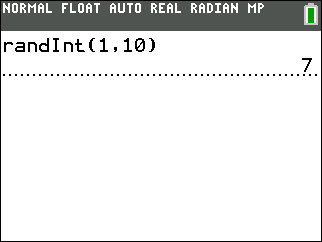
\includegraphics[width=0.4\linewidth]{images/randInt-single.png}
\end{figure}\end{computation}
\begin{computation}{List of Random Integers.}{computation-2}%
\hypertarget{p-11}{}%
To generate a list of 4 random integers between 1 and 10:\leavevmode%
\begin{enumerate}
\item\hypertarget{li-5}{}Press the \mono{math} button and use the cursor to highlight the \mono{PROB} tab.%
\item\hypertarget{li-6}{}Select \mono{5:randInt(}%
\item\hypertarget{li-7}{}Fill out the StatWizard so it looks like below%
\begin{codedisplay}

		      lower:1
		      upper:10
		      n:4
		      Paste
		    
\end{codedisplay}
Highlight \mono{Paste} and press \mono{enter}.%
\item\hypertarget{li-8}{}Press \mono{enter} to execute the function you previously pasted into the command window.%
\end{enumerate}
%
\begin{figure}\centering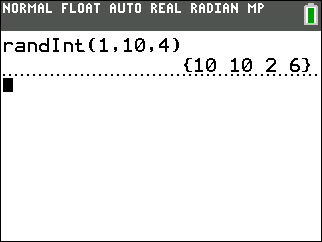
\includegraphics[width=0.4\linewidth]{images/randInt-list.png}
\end{figure}\end{computation}
\begin{computation}{List of Random Integers with No Repeats.}{computation-3}%
\hypertarget{p-12}{}%
To generate a list of 10 random integers between 1 and 20 with \emph{no repeats}:\leavevmode%
\begin{enumerate}
\item\hypertarget{li-9}{}Press the \mono{math} button and use the cursor to highlight the \mono{PROB} tab.%
\item\hypertarget{li-10}{}Select \mono{8:randIntNoRep(}%
\item\hypertarget{li-11}{}Fill out the StatWizard so it looks like below%
\begin{codedisplay}

		      lower:1
		      upper:20
		      n:10
		      Paste
		    
\end{codedisplay}
Highlight \mono{Paste} and press \mono{enter}.%
\item\hypertarget{li-12}{}Press \mono{enter} to execute the function you previously pasted into the command window.%
\end{enumerate}
%
\begin{figure}\centering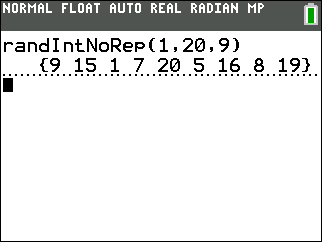
\includegraphics[width=0.4\linewidth]{images/randIntNoRep.png}
\end{figure}\end{computation}
\end{subsectionptx}
%
%
\typeout{************************************************}
\typeout{Reading Questions 1.3.2 Four Tickets for Friends}
\typeout{************************************************}
%
\begin{reading-questions-subsection}{Four Tickets for Friends}{}{Four Tickets for Friends}{}{}{reading-questions-9}
\hypertarget{p-13}{}%
Sophia has 10 friends that she would like to invite to a concert, but only 4 tickets to give away.%
\par
\hypertarget{p-14}{}%
Mike, Jamie, Adam, Yvette, Ashley, Monica, Cherie, Julie, Willard, Bruce%
\begin{divisionexercise}{1}{}{}{exercise-38}%
Which of the following would produce a simple random sample of the 4 friends that she will bring with her: \leavevmode%
\begin{enumerate}[label=(\alph*)]
\item\hypertarget{li-13}{}List each persons name on a piece of paper, place them in a hat and draw 4. \textbf{Answer}.\quad%
yes%
\item\hypertarget{li-14}{}List the names in alphabetical order and take the first 4 names. \textbf{Answer}.\quad%
no%
\item\hypertarget{li-15}{}Ask one of her friends who she should bring. \textbf{Answer}.\quad%
no%
\item\hypertarget{li-16}{}Number the friends from 1 to 10 and use a random number generator to produce 4 numbers between 1 and 10 which correspond to the 10 friends. \textbf{Answer}.\quad%
yes%
\end{enumerate}
\end{divisionexercise}%
\begin{divisionexercise}{2}{}{}{exercise-39}%
Use the TI graphing calculator to obtain a random sample of the 4 friends that she will bring with her and give their names. \textbf{Solution}.\hypertarget{solution-1}{}\quad%
\begin{figure}\centering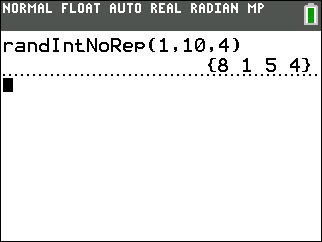
\includegraphics[width=0.4\linewidth]{images/four-friends.png}
\end{figure}\hypertarget{p-15}{}%
Thus she would invite Mike, Yvette, Ashley and Julie.%
\par
\hypertarget{p-16}{}%
We can also have the calculator sort the list in ascending order:%
\begin{figure}\centering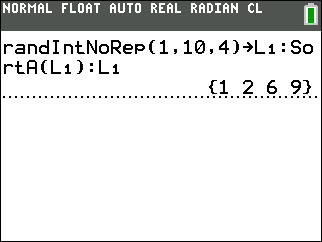
\includegraphics[width=0.4\linewidth]{images/four-friends-sorted.png}
\end{figure}\hypertarget{p-17}{}%
In this case, she would invite Mike, Jamie, Monica and Willard.%
\end{divisionexercise}%
\end{reading-questions-subsection}
%
%
\typeout{************************************************}
\typeout{Reading Questions 1.3.3 Employee Survey}
\typeout{************************************************}
%
\begin{reading-questions-subsection}{Employee Survey}{}{Employee Survey}{}{}{reading-questions-10}
\hypertarget{p-18}{}%
The owner of a private food store is concerned with employee morale. She decides to survey the employees to learn about work environment and job satisfaction. \begin{tabular}{llll}\hrulethick
1 Archer&9 Foushi&16 Kemp&23 Oliver\tabularnewline\hrulethin
2 Bolcerek&10 Gow&17 Lathus&24 Orsini\tabularnewline\hrulethin
3 Bryant&11 Grove&18 Lindsey&25 Salazar\tabularnewline\hrulethin
4 Carlisle&12 Hall&19 Massie&26 Ullrich\tabularnewline\hrulethin
5 Cole&13 Hills&20 McGuffin&27 Vaneck\tabularnewline\hrulethin
6 Dimas&14 Houston&21 Musa&28 Weber\tabularnewline\hrulethin
7 Ellison&15 Kats&22 Nickas&29 Zavodny\tabularnewline\hrulethin
8 Everhart&&&\tabularnewline\hrulethick
\end{tabular}
%
\begin{divisionexercise}{1}{}{}{exercise-40}%
Obtain a simple random sample of size 6 from the above table using the TI graphing calculator. \textbf{Solution}.\hypertarget{solution-2}{}\quad%
\begin{figure}\centering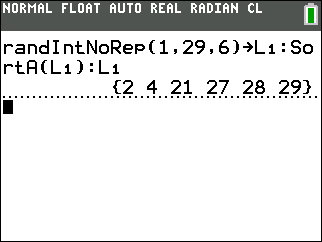
\includegraphics[width=0.4\linewidth]{images/employee-survey.png}
\end{figure} Thus the randomly selected employees are: Bolcerek, Carlisle, Musa, Vaneck, Weber, and Zavodny.\end{divisionexercise}%
\end{reading-questions-subsection}
\end{sectionptx}
%
%
\typeout{************************************************}
\typeout{Section 1.4 Other Effective Sampling Methods}
\typeout{************************************************}
%
\begin{sectionptx}{Other Effective Sampling Methods}{}{Other Effective Sampling Methods}{}{}{sec-other-sampling-methods}
\begin{definition}{stratified sampling.}{definition-32}%
a simple random sample is drawn from each nonoverlapping subgroup (or \terminology{stratum}) into which the population has been separated.\hypertarget{p-19}{}%
Works best when individuals in each stratum are similar in some way and we want to make sure each stratum type is represented. The size of each simple random sample is proportional to the number of individuals in the stratum from which it is selected. (e.g.\@ separating individuals into age groups)%
\end{definition}
\begin{definition}{systematic sampling.}{definition-33}%
\hypertarget{p-20}{}%
a starting point, \(p\), is randomly selected and then every \(k\)th subject is included in the sample, where%
\begin{gather*}
k = \lfloor N/n \rfloor
\end{gather*}
The brackets, \(\lfloor x \rfloor\), mean round \(x\) down to the nearest integer, or take the \terminology{floor} of \(x\). Subjects in the sample are numbered:%
\begin{gather*}
p, p+k, p+2k, p+3k, \ldots, p+(n-1)k
\end{gather*}
%
\par
\hypertarget{p-21}{}%
Works best when individuals are arranged sequentially but you’re not sure how many total individuals there are because you don’t have a frame of the population (files in a drawer, people coming out of a building e.g.\@ exit polling, etc.\@).%
\end{definition}
\begin{definition}{cluster sampling.}{definition-34}%
\hypertarget{p-22}{}%
the population is divided into sections or \terminology{clusters}; all individuals from randomly selected clusters are included in the sample.%
\par
\hypertarget{p-23}{}%
Works best when individuals are grouped geographically so it makes logistical sense to sample this way, but location does not affect your variable of interest; clusters are heterogeneous like the population.%
\end{definition}
\begin{definition}{convenience sampling.}{definition-35}%
\hypertarget{p-24}{}%
sampling subjects who are easy to get (bad sampling method).%
\par
\hypertarget{p-25}{}%
Works best when: NEVER!! (not random)%
\end{definition}
\begin{definition}{self-selected.}{definition-36}%
\hypertarget{p-26}{}%
a convenience sample where individuals are self-selected (another bad sampling method).%
\par
\hypertarget{p-27}{}%
Works best when: NEVER!! (not random, favors those with stronger opinions)%
\end{definition}
\begin{definition}{multi-stage sample.}{definition-37}%
\hypertarget{p-28}{}%
a sample that is selected in multiple stages, each of which might use a different method of sampling.%
\par
\hypertarget{p-29}{}%
Works best when: The population is organized hierarchically but no list exists.%
\end{definition}
\end{sectionptx}
%
%
\typeout{************************************************}
\typeout{Section 1.5 Bias in Sampling}
\typeout{************************************************}
%
\begin{sectionptx}{Bias in Sampling}{}{Bias in Sampling}{}{}{sec-bias-in-sampling}
\hypertarget{p-30}{}%
Lorem ipsum dolor sit amet, consectetur adipiscing elit. Fusce tincidunt lectus nec gravida mattis. Donec viverra bibendum felis, in egestas neque commodo vel. Duis id consectetur sapien. Etiam vel ante ut quam fringilla faucibus. Pellentesque a dictum enim, sed molestie quam. Morbi finibus facilisis orci, a tempor quam hendrerit sit amet. Phasellus eget maximus enim. Pellentesque fermentum nulla lectus, sed blandit risus tempus sed. Praesent bibendum facilisis maximus. Fusce vestibulum nulla in tincidunt vulputate. Sed at velit non orci molestie vulputate. Donec auctor risus vel purus auctor laoreet quis a mi. In eget tempor quam.%
\end{sectionptx}
\end{chapterptx}
\end{partptx}
%
%
\typeout{************************************************}
\typeout{Part II Descriptive Statistics}
\typeout{************************************************}
%
\begin{partptx}{Descriptive Statistics}{}{Descriptive Statistics}{}{}{part-descriptive-stats}
 %
%
\typeout{************************************************}
\typeout{Chapter 2 Summarizing Data in Tables and Graphs}
\typeout{************************************************}
%
\begin{chapterptx}{Summarizing Data in Tables and Graphs}{}{Summarizing Data in Tables and Graphs}{}{}{ch-tables-and-graphs}
%
%
\typeout{************************************************}
\typeout{Section 2.1 Organizing Qualitative Data}
\typeout{************************************************}
%
\begin{sectionptx}{Organizing Qualitative Data}{}{Organizing Qualitative Data}{}{}{sec-organizing-qualitative-data}
\hypertarget{p-31}{}%
Placeholder text%
\end{sectionptx}
%
%
\typeout{************************************************}
\typeout{Section 2.2 Organizing Quantitative Data}
\typeout{************************************************}
%
\begin{sectionptx}{Organizing Quantitative Data}{}{Organizing Quantitative Data}{}{}{sec-organizing-quantitative-data}
\hypertarget{p-32}{}%
Placeholder text%
\end{sectionptx}
%
%
\typeout{************************************************}
\typeout{Section 2.3 Graphical Misrepresentations of Data}
\typeout{************************************************}
%
\begin{sectionptx}{Graphical Misrepresentations of Data}{}{Graphical Misrepresentations of Data}{}{}{sec-graphical-misrepresentations-of-data}
\hypertarget{p-33}{}%
Placeholder text%
\end{sectionptx}
\end{chapterptx}
 %
%
\typeout{************************************************}
\typeout{Chapter 3 Numerically Summarizing Data}
\typeout{************************************************}
%
\begin{chapterptx}{Numerically Summarizing Data}{}{Numerically Summarizing Data}{}{}{ch-numerical-summaries}
%
%
\typeout{************************************************}
\typeout{Section 3.1 Measures of Central Tendency}
\typeout{************************************************}
%
\begin{sectionptx}{Measures of Central Tendency}{}{Measures of Central Tendency}{}{}{sec-measures-central-tendency}
\hypertarget{p-34}{}%
Placeholder text%
\end{sectionptx}
%
%
\typeout{************************************************}
\typeout{Section 3.2 Measures of Dispersion}
\typeout{************************************************}
%
\begin{sectionptx}{Measures of Dispersion}{}{Measures of Dispersion}{}{}{sec-measures-dispersion}
\hypertarget{p-35}{}%
Placeholder text%
\end{sectionptx}
%
%
\typeout{************************************************}
\typeout{Section 3.3 Measures of Central Tendency and Dispersion from Grouped Data}
\typeout{************************************************}
%
\begin{sectionptx}{Measures of Central Tendency and Dispersion from Grouped Data}{}{Measures of Central Tendency and Dispersion from Grouped Data}{}{}{sec-measures-grouped-data}
\hypertarget{p-36}{}%
Placeholder text%
\end{sectionptx}
%
%
\typeout{************************************************}
\typeout{Section 3.4 Measures of Position and Outliers}
\typeout{************************************************}
%
\begin{sectionptx}{Measures of Position and Outliers}{}{Measures of Position and Outliers}{}{}{sec-measures-position-and-outliers}
\hypertarget{p-37}{}%
Placeholder text%
\end{sectionptx}
%
%
\typeout{************************************************}
\typeout{Section 3.5 The Five-{}-{}Number Summary and Boxplots}
\typeout{************************************************}
%
\begin{sectionptx}{The Five-{}-{}Number Summary and Boxplots}{}{The Five-{}-{}Number Summary and Boxplots}{}{}{sec-five-number-summary-boxplots}
\hypertarget{p-38}{}%
Placeholder text%
\end{sectionptx}
\end{chapterptx}
 %
%
\typeout{************************************************}
\typeout{Chapter 4 Describing the Relation between Two Variables}
\typeout{************************************************}
%
\begin{chapterptx}{Describing the Relation between Two Variables}{}{Describing the Relation between Two Variables}{}{}{ch-relations-between-two-varibles}
\end{chapterptx}
\end{partptx}
%
%
\typeout{************************************************}
\typeout{Part III Probability and Probability Distributions}
\typeout{************************************************}
%
\begin{partptx}{Probability and Probability Distributions}{}{Probability and Probability Distributions}{}{}{part-probability}
 %
%
\typeout{************************************************}
\typeout{Chapter 5 Probability}
\typeout{************************************************}
%
\begin{chapterptx}{Probability}{}{Probability}{}{}{ch-probability}
\end{chapterptx}
 %
%
\typeout{************************************************}
\typeout{Chapter 6 Discrete Probability Distributions}
\typeout{************************************************}
%
\begin{chapterptx}{Discrete Probability Distributions}{}{Discrete Probability Distributions}{}{}{ch-discrete-probability}
\end{chapterptx}
 %
%
\typeout{************************************************}
\typeout{Chapter 7 The Normal Probability Distribution}
\typeout{************************************************}
%
\begin{chapterptx}{The Normal Probability Distribution}{}{The Normal Probability Distribution}{}{}{ch-normal-probability}
\end{chapterptx}
\end{partptx}
%
%
\typeout{************************************************}
\typeout{Part IV Inference: From Samples to Population}
\typeout{************************************************}
%
\begin{partptx}{Inference: From Samples to Population}{}{Inference: From Samples to Population}{}{}{part-inferential-stats}
 %
%
\typeout{************************************************}
\typeout{Chapter 8 Sampling Distributions}
\typeout{************************************************}
%
\begin{chapterptx}{Sampling Distributions}{}{Sampling Distributions}{}{}{ch-sampling-distributions}
\end{chapterptx}
 %
%
\typeout{************************************************}
\typeout{Chapter 9 Estimating the Value of a Parameter}
\typeout{************************************************}
%
\begin{chapterptx}{Estimating the Value of a Parameter}{}{Estimating the Value of a Parameter}{}{}{ch-estimating-parameters}
\end{chapterptx}
 %
%
\typeout{************************************************}
\typeout{Chapter 10 Hypothesis Tests Regarding a Parameter}
\typeout{************************************************}
%
\begin{chapterptx}{Hypothesis Tests Regarding a Parameter}{}{Hypothesis Tests Regarding a Parameter}{}{}{ch-hypothesis-tests}
\end{chapterptx}
 %
%
\typeout{************************************************}
\typeout{Chapter 11 Inferences on Two Samples}
\typeout{************************************************}
%
\begin{chapterptx}{Inferences on Two Samples}{}{Inferences on Two Samples}{}{}{ch-inferences-on-two-samples}
\end{chapterptx}
\end{partptx}
\end{document}